\documentclass[tikz]{standalone}
\usepackage{bm}
\newcommand{\vect}{\bm}
\newcommand{\del}{\boldsymbol{\nabla}}

\begin{document}
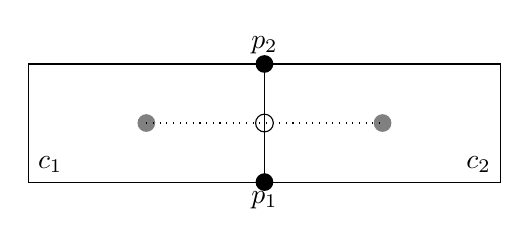
\begin{tikzpicture}[
  scale=0.75,
  cpnt/.style={fill=gray},
  vertex/.style={fill=black},
  arr/.style={thick, <->},
  mag/.style={dashed, thick, <->}
]
\draw (0,0) rectangle (4,2);
\draw (4,2) -- (8,2) -- (8,0) -- (4,0);
\path [vertex] (4,0) circle [radius=0.15] node [below] {$p_1$};
\path [vertex] (4,2) circle [radius=0.15] node [above] {$p_2$};
\node [above right] at (0,0) {$c_1$};
\node [above left] at (8,0) {$c_2$};

\path [cpnt] (2,1) circle [radius=0.15];
\path [cpnt] (6,1) circle [radius=0.15];
\draw [dotted] (2,1) -- (6,1);
\draw (4,1) circle [radius=0.15];
\end{tikzpicture}
\end{document}
